\documentclass[twoside]{article}
\usepackage{geometry}
\geometry{paperwidth=148mm,paperheight=210mm,margin=15mm}
\usepackage{graphicx}
\usepackage{stix}
\usepackage{url}
\usepackage{natbib}
\usepackage{booktabs}
%\pagestyle{empty}\thispagestyle{empty}

\title{Compact notes on probability and statistics}
\author{Erik Ø. Sørensen}

% List of newcommands used in
% ``Notation in Econometrics:
% A Proposal for a Standard''
% by Karim Abadir and Jan Magnus
% Med et lite tillegg av Erik �. S�rensen: \defdas
%
\usepackage{amsfonts}
%\usepackage{amssymb}
\usepackage{graphics}
\usepackage{epsfig}
\usepackage{verbatim}

\usepackage{latexsym}
\usepackage{amsmath}
%%%
\newcommand{\newoperator}[3]{\newcommand*{#1}{\mathop{#2}#3}}
\newcommand{\renewoperator}[3]{\renewcommand*{#1}{\mathop{#2}#3}}
%
% Dette er min egen:
\newcommand{\defdas}{\mathrel{\raise0.095ex\hbox{$:$}\mkern-5mu = }}
%
% symbols C,N,Q,R,Z for sets
\newcommand{\SC}{\mathbb{C}}
\newcommand{\SN}{\mathbb{N}}
\newcommand{\SQ}{\mathbb{Q}}
\newcommand{\SR}{\mathbb{R}}
\newcommand{\SZ}{\mathbb{Z}}
%
% calligraphic capital letters
\newcommand{\calA}{\mathcal{A}}
\newcommand{\calB}{\mathcal{B}}
\newcommand{\calC}{\mathcal{C}}
\newcommand{\calD}{\mathcal{D}}
\newcommand{\calE}{\mathcal{E}}
\newcommand{\calF}{\mathcal{F}}
\newcommand{\calG}{\mathcal{G}}
\newcommand{\calH}{\mathcal{H}}
\newcommand{\calI}{\mathcal{I}}
\newcommand{\calJ}{\mathcal{J}}
\newcommand{\calK}{\mathcal{K}}
\newcommand{\calL}{\mathcal{L}}
\newcommand{\calM}{\mathcal{M}}
\newcommand{\calN}{\mathcal{N}}
\newcommand{\calO}{\mathcal{O}}
\newcommand{\calP}{\mathcal{P}}
\newcommand{\calQ}{\mathcal{Q}}
\newcommand{\calR}{\mathcal{R}}
\newcommand{\calS}{\mathcal{S}}
\newcommand{\calT}{\mathcal{T}}
\newcommand{\calU}{\mathcal{U}}
\newcommand{\calV}{\mathcal{V}}
\newcommand{\calW}{\mathcal{W}}
\newcommand{\calX}{\mathcal{X}}
\newcommand{\calY}{\mathcal{Y}}
\newcommand{\calZ}{\mathcal{Z}}
%
% bold lowercase and capital letters for vectors (v) and matrices (m)
\newcommand{\mA}{\bm A}
\newcommand{\va}{\bm a}
\newcommand{\mB}{\bm B}
\newcommand{\vb}{\bm b}
\newcommand{\mC}{\bm C}
\newcommand{\vc}{\bm c}
\newcommand{\mD}{\bm D}
\newcommand{\vd}{\bm d}
\newcommand{\mE}{\bm E}
\newcommand{\ve}{\bm e}
\newcommand{\mF}{\bm F}
\newcommand{\vf}{\bm f}
\newcommand{\mG}{\bm G}
\newcommand{\vg}{\bm g}
\newcommand{\mH}{\bm H}
\newcommand{\vh}{\bm h}
\newcommand{\mI}{\bm I}
\newcommand{\vi}{\bm i}
\newcommand{\mJ}{\bm J}
\newcommand{\vj}{\bm j}
\newcommand{\mK}{\bm K}
\newcommand{\vk}{\bm k}
\newcommand{\mL}{\bm L}
\newcommand{\vl}{\bm l}
\newcommand{\mM}{\bm M}
\newcommand{\vm}{\bm m}
\newcommand{\mN}{\bm N}
\newcommand{\vn}{\bm n}
\newcommand{\mO}{\bm O}
\newcommand{\vo}{\bm o}
\newcommand{\mP}{\bm P}
\newcommand{\vp}{\bm p}
\newcommand{\mQ}{\bm Q}
\newcommand{\vq}{\bm q}
\newcommand{\mR}{\bm R}
\newcommand{\vr}{\bm r}
\newcommand{\mS}{\bm S}
\newcommand{\vs}{\bm s}
\newcommand{\mT}{\bm T}
\newcommand{\vt}{\bm t}
\newcommand{\mU}{\bm U}
\newcommand{\vu}{\bm u}
\newcommand{\mV}{\bm V}
\newcommand{\vv}{\bm v}
\newcommand{\mW}{\bm W}
\newcommand{\vw}{\bm w}
\newcommand{\mX}{\bm X}
\newcommand{\vx}{\bm x}
\newcommand{\mY}{\bm Y}
\newcommand{\vy}{\bm y}
\newcommand{\mZ}{\bm Z}
\newcommand{\vz}{\bm z}
%
% bold Greek lowercase letters for vectors (v)
\newcommand{\valpha}{\bm \alpha}
\newcommand{\vbeta}{\bm \beta}
\newcommand{\vgamma}{\bm \gamma}
\newcommand{\vdelta}{\bm \delta}
\newcommand{\vepsi}{\bm \epsi}
\newcommand{\vvarepsilon}{\bm \varepsilon}
\newcommand{\vzeta}{\bm \zeta}
\newcommand{\veta}{\bm \eta}
\newcommand{\vtheta}{\bm \theta}
\newcommand{\viota}{\bm \iota}
\newcommand{\vkappa}{\bm \kappa}
\newcommand{\vlambda}{\bm \lambda}
\newcommand{\vmu}{\bm \mu}
\newcommand{\vnu}{\bm \nu}
\newcommand{\vxi}{\bm \xi}
\newcommand{\vpi}{\bm \pi}
\newcommand{\vrho}{\bm \rho}
\newcommand{\vsigma}{\bm \sigma}
\newcommand{\vtau}{\bm \tau}
\newcommand{\vupsilon}{\bm \upsilon}
\newcommand{\vphi}{\bm \phi}
\newcommand{\vchi}{\bm \chi}
\newcommand{\vpsi}{\bm \psi}
\newcommand{\vomega}{\bm \omega}
%
% bold Greek capital letters for matrices (m)
\newcommand{\mGamma}{\bm \varGamma}
\newcommand{\mDelta}{\bm \varDelta}
\newcommand{\mTheta}{\bm \varTheta}
\newcommand{\mLambda}{\bm \varLambda}
\newcommand{\mXi}{\bm \varXi}
\newcommand{\mPi}{\bm \varPi}
\newcommand{\mSigma}{\bm \varSigma}
\newcommand{\mUpsilon}{\bm \varUpsilon}
\newcommand{\mPhi}{\bm \varPhi}
\newcommand{\mPsi}{\bm \varPsi}
\newcommand{\mOmega}{\bm \varOmega}
%
% roman letters in mathematics
\newcommand{\rB}{\ensuremath{\mathrm{B}}}
\newcommand{\rC}{\ensuremath{\mathrm{C}}}
\newcommand{\rD}{\ensuremath{\mathrm{D}}}
\newcommand{\rF}{\ensuremath{\mathrm{F}}}
\newcommand{\rH}{\ensuremath{\mathrm{H}}}
\newcommand{\rL}{\ensuremath{\mathrm{L}}}
\newcommand{\rN}{\ensuremath{\mathrm{N}}}
\newcommand{\rt}{\ensuremath{\mathrm{t}}}
\newcommand{\rU}{\ensuremath{\mathrm{U}}}
%
\newcommand{\bin}{\ensuremath{\mathrm{bin}}}
\newcommand{\eu}{\ensuremath{\mathrm{e}}}
\newcommand{\iu}{\ensuremath{\mathrm{i}}}
\newcommand{\LN}{\ensuremath{\mathrm{LN}}}
\newcommand{\Po}{\ensuremath{\mathrm{Po}}}
%
\newcommand{\ped}[1]{\ensuremath{_\mathrm{#1}}} %pedex
\newcommand{\ap}[1]{\ensuremath{^\mathrm{#1}}} %apex
\renewoperator{\Re}{\mathrm{Re}}{\nolimits}
\renewoperator{\Im}{\mathrm{Im}}{\nolimits}
%
% letters for (partial) differentiation
%\newcommand{\rd}{\ensuremath{\mathrm{d}}}
\makeatletter
\newcommand{\rd}{\@ifnextchar^{\DIfF}{\DIfF^{}}}
\def\DIfF^#1{%
   \mathop{\mathrm{\mathstrut d}}%
   \nolimits^{#1}\gobblespace}
\def\gobblespace{\futurelet\diffarg\opspace}
\def\opspace{%
   \let\DiffSpace\!%
   \ifx\diffarg(%
   \let\DiffSpace\relax
   \else
   \ifx\diffarg[%
   \let\DiffSpace\relax
   \else
   \ifx\diffarg\{%
   \let\DiffSpace\relax
   \fi\fi\fi\DiffSpace}
\newcommand{\deriv}[3][]{\frac{\rd^{#1}#2}{\rd #3^{#1}}}
\newcommand{\pderiv}[3][]{\frac{\partial^{#1}#2}{\partial #3^{#1}}}
%
% operatornames
\newcommand{\bias}{\operatorname{bias}}
\newcommand{\col}{\operatorname{col}}
\newcommand{\corr}{\operatorname{corr}}
\newcommand{\cov}{\operatorname{cov}}
\newcommand{\dg}{\operatorname{dg}}
\newcommand{\diag}{\operatorname{diag}}
\newcommand{\E}{\operatorname{E}}
\newcommand{\etr}{\operatorname{etr}}
\newoperator{\ip}{\mathrm{int}}{\nolimits}
\newcommand{\kur}{\operatorname{kur}}
\newcommand{\median}{\operatorname{med}}
\newcommand{\MSE}{\operatorname{MSE}}
\newcommand{\plim}{\operatorname{plim}}
\newcommand{\rk}{\operatorname{rk}}
\newcommand{\sgn}{\operatorname{sgn}}
\newcommand{\tr}{\operatorname{tr}}
\newcommand{\var}{\operatorname{var}}
\renewcommand{\vec}{\operatorname{vec}}
\newcommand{\vech}{\operatorname{vech}}
%
% other definitions
\newcommand{\distr}{\sim}
\newcommand{\adistr}{\stackrel{a}{\distr}}
\newcommand{\diff}{\bigtriangledown}
\newcommand{\fordiff}{\bigtriangleup}
\newcommand{\mply}{\cdot}
\newcommand{\widebar}{\overline}
%
%\mathchardef\varepsilon="010F
%\mathchardef\epsilon="0122
%\mathchardef\eps="010F
\newcommand{\eps}{\epsilon}
\newcommand{\epsi}{\varepsilon}
%
\newcommand{\longto}{\longrightarrow}
\newcommand{\pto}{\stackrel{p}{\longrightarrow}}
\newcommand{\dto}{\stackrel{d}{\longrightarrow}}
\newcommand{\wto}{\stackrel{w}{\longrightarrow}}
%
\newcommand{\vvarsigma}{\bm \varsigma}
\newcommand{\score}{\vvarsigma}
\newcommand{\Infmat}{\bm\calI}
\newcommand{\Hesmat}{\bm\calH}
%
\newcommand{\vones}{\bm\imath}
\newcommand{\vzeros}{\boldsymbol{0}}
\newcommand{\mzeros}{\mathbf{O}}
%
\newcommand{\bcdot}{\raisebox{1pt}{\textbf{\large .}}}
\newcommand{\interior}[1]{\overset{\circ}{#1}}
%
\newcommand{\hspacesymbols}%
   {$\{x: x \in S, x$ satisfies $P\}\;\;$} %symbols index
\newcommand{\type}[1]{{\tt$\backslash$#1}}

\usepackage{bm}

%\theoremstyle{theorem}
\newtheorem{theorem}{Theorem}%[section]
\begin{document}
\maketitle
\sloppy
\frenchspacing



\tableofcontents
\thispagestyle{empty}
\newpage
\noindent This set of compact notes is written to support the August method camp
in probability and statistics for new PhD students at NHH Norwegian School of
Economics, and is in no way intended to replace a proper book on the topics or
be subject to independent study.

This set of notes relies a lot on the two books
I have used for teaching in the last decade: \citet{Hogg2013} and
\citet{Linton2017}. When it comes to the statistics part, econometrics textbooks
will probably be sufficient for almost everyone. For those that need a more
theoretical grounding, a first escalation might be \citet{Rosenthal2006}; the
level of rigour of \citet{Billingsley1995} should be sufficiently high for
everyone.


We will not cover software in the Method Camp, but you can never go wrong by
having a look at \citet{Wickham2017} and their introduction to modern~R.


\section{Probability}
Modern probability theory (since the 1930s) is defined in terms of set theoretic
notions. 
Let us define a \textbf{sample space} of all possible outcome of some
event (a set). Example, role of a die: $\calS =\{1,2,3,4,5,6\}$. 
An \textbf{event} is a subset of $\calS$. Events are what we assign probability
to.

The set of possible events must be restricted to a
$\mathbf{\sigma}$\textbf{-algebra} $\calA$, a class of subsets of $\calS$. We
require that if $A\in\calS$ then $A^c\in\calA$; if $A\in\calA$ and $B\in\calA$
then $A\cup B$ is also in $\calA$. This defines an \textbf{algebra}. We also
require that taking  if $A_1,A_2,\dots\in \calA$, then $\cup_{i=1}^\infty A_i
\in \calA$, this last requirement is what restricts $\calA$ to a
$\sigma$-algebra. Some authors reference a $\sigma$-algebra as a $\sigma$-\emph{field}.

$P$ is a \textbf{probability set function} if $P(A)\geq0$ for all $A\in\calA$; $P(\emptyset)=0$; $P(\calS)=1$,
and if $A_1,A_2,\dots$ is a series of \textbf{disjoint} sets ($A_i\cap A_j\emptyset$ when $i\neq j$), then
$P(\cup_{i=1}^\infty A_i)=\sum_{i=1}^\infty P(A_i)$. 
The triple $(\calS,\calA,P)$ is called a \textbf{probability space}.

With a discrete sample space, we will often work with the set of all subsets as the relevant 
$\sigma$-algebra. The set of all subsets is also referred to as the \textbf{power set} and written $2^\calS$.
If the sample space is continuous (like the set of all real numbers), there are technical difficulties
working with the power set; the power set of $\SR$ is not a $\sigma$-algebra. Instead, for real numbers 
we work with subsets that are open intervals, $\calB = \{(a,b), \ a,b\in\SR\}$. Using all sets of type $\calB$,
and the countable unions and complements of these sets, we can define the \textbf{Borel $\sigma$-algebra}.

For $A$ and $B$ in $\calA$, we define the \textbf{conditional probability} of $A$ given $B$
as \[ P(A|B) = P(A\cap B)/P(B),\] when $P(B)>0$. From the definition, we can find 
\textbf{Bayes rule}
as 
\[ P(B|A) = \frac{ P(A|B)\cdot P(B)}{P(A)}.\]

If $A$ and $B$ are events with positive probability, $A$ and $B$ are \textbf{independent} if
$P(A\cap B) = P(A)\cdot P(B)$, $P(A|B)=P(A)$, and $P(B|A)=P(B)$ (all equivalent). Independence
is symmetric but not transitive.

\section{Random variables}

A \textbf{random variable}  (r.v.) is a function from a sample space to the real numbers,
$X\!\!: \calS \rightarrow \SR$. The probability space on $\calS$ maps to a new
probability space on $\SR$. There are technical requirements:
$X$ must be \textbf{measurable},
\[ \calA_X = \{A\subset S: X(A) \in \calB\} = \{X^{-1}(B): B\in \calB\}\subseteq \calA.\]
Here $\calB$ is a $\sigma$-algebra on $\SR$ and $\calA$ is the $\sigma$-algebra on $\calS$.
Now the probability measure $P_X$ is defined $P_X(B) = P(X^{-1}(B))$.

It is customary to use capital roman letters to refer to random variables, but
lower case letters to refer to particular values (numbers), such that $X(s)=x$
is the statement that at $s\in\calS$, the random variable $X$ takes on the value $x$.

\subsection{Distribution}
A random variable $X$ is said to have a \textbf{distribution function} (d.f.) $F_X$
such that \[ F_X(s) = P_X((-\infty, s])=P(\{a: X(a)\leq s\}).\] When the derivative of the
distribution function exists, it is called the \textbf{density} of $X$, and
$f_X(s)=F'_X(s)$. We then say $X$ is distributed \textbf{continuously}. General
properties: $f_X(s)\geq0$, $\int_a^b f_X(s)\rd s = P(X\in[a,b])$, and
$\int_{-\infty}^\infty f_X(s) \rd s = 1$. When clear from context, we drop the
subscripts (and sometimes also the limits of integration): $\int\! f(s)\rd s=1$.

For \textbf{discrete} r.v., we define the \textbf{probability mass function} (pmf) as
$p_X(s) = P(X\in\{s\})$ for $s\in\calS$. This is analogous to the density function.

\subsection{Expectation of a random variable}
Let $X$ be a random variable. If $X$ is a continuous r.v.
with pdf $f(x)$ and 
\(\int_{-\infty}^\infty |x|f(x) \rd x < \infty,\)
the \textbf{expectation} of $X$ exists as  
\[\E[X] = \int_{-\infty}^\infty xf(x) \rd x.\]
If $Y$ is a discrete random variable with pmf $p_Y$, 
$\E[Y]=\sum_y yp_Y(y)$.

Having different expressions for discrete and continuous random variables is awkward, since
sometimes we need to do theory for mixed variables or variables where we don't know the 
distribution. To find a more general way to express expectations, we need to extend
our notion of \emph{integration}, this is outside the scope of our method camp. But we sometimes
see expressions such at $\E[X]=\int\! x \rd F_X(x)$
or even $E[X]=\int_\Omega X(\omega) P(\rd \omega)$.

The k-th \textbf{moment} of $X$ is $\E [X^k]$ (when it exists).  We often write $\mu=\E[X]$ (the \textbf{mean}) and
$\sigma^2 = \E[(X-\mu)^2]$ (the \textbf{variance}). The k-th \textbf{central moment} 
is $\E [ (X-\mu)^k]$.

The function expectation $m_X(t)=\E[e^{tX}]$ is called the \textbf{moment generating function}
when it exists in an open ball around zero. When it exists, $m'(0)=\E[X]$, $m''(0)=\E[X^2]$ and
$m^k(0)=\E[X^k]$.

\subsection{Expectation results}
\begin{enumerate}
\item Let $X$ be a random variable and let $m$ be a positive integer. 
Suppos(e that $E[X^m]$ exists. If $k$ is an integer and $k < m$, then
$E[X^k]$ exists.
\item Let $u(X)$ be a nonnegative function of the random variable $X$. If
$E[u(X)]$ exists, then for every positive constant $c$,
$P(u(X)\geq c) \leq \frac{E[u(X)]}{c}$ (\textbf{Markov}).
\item Let the random variable $X$ have a distribution with
finite variance $\sigma^2$. Then for every $k>0$, 
$P(|X-\mu|\geq k\sigma) \leq \frac{1}{k^2}$ (\textbf{Chebyshev}).
\item If $\phi$ is convex on an open interval $I$ and $X$ is a random
variable whose support is contained in $I$ and has finite expectation,
then $ \phi(E[X]) \leq E[\phi(X)]$ (\textbf{Jensen}).
\end{enumerate}

\subsection{Common distributions}
There are some distributions we are expected to know about:

\begin{description}
\item[Uniform] A uniform distribution on $[a,b]$ is written $U(a,b)$, has a density $1/(b-a)$ on $[a,b]$ and 
a d.f. $F(x)=x/(b-a)$ on $[a,b]$. 
\item[Standard normal] A standard normal distribution is written $N(0,1)$, and the density is 
\[ \phi(z) = \frac{1}{\sqrt{2\pi}} e^{-z^2/2}.\] The distribution function is often written $\Phi(z)$ but
there is no analytical expression. See Table~\ref{tab:z} in the back for some tabulated values.
The moment generating function is $m(t) = \exp(t^2/2)$.
\item[Exponential] An exponential distribution with parameter $\lambda$ is written $\mathrm{Exp}(\lambda)$, 
has density $f(x)=\lambda \exp(-\lambda  x)$ on $[0,\infty)$, and distribution function $F(x)=1- \exp(-\lambda x)$.
\item[Binomial] If an event happens with probability $p$ in a single (binary)
Bernoulli trial, the distribution of the number of events $k$ in $n$ trials has
probability mass function $p(k) = \binom{n}{k} p^k (1-p)^{n-k}$ (with the
binomial coefficient $\binom{n}{k} = n!/k!(n-k)!$).
\item[Poisson] A Poisson distribution on the integers $\{0,1,2,\dots\}$ has probability mass function 
$p(x) = \lambda^x \exp(-\lambda)/x!$, the distribution function is not pretty. The moment generating function
is $m(t) = \exp(\lambda( \exp(t) -1))$.
\end{description}

A more complete overview of distributions is given by \citet{Leemis2008}.

\subsection{Functions of random variables}
If $X$ is a random variable and $g$ is a function, $Y=g(X)$ is another random variable.

In Figure~\ref{fig:frv}a, $Y=g(x)$ is an increasing function. 
Thinking about the distribution of $Y$, if we start from the primitives,
the distribution function for $Y$ is $F_Y(y) = P(Y\leq y)$. We can substitute
the definition of $Y$ into this: $F_Y(y) = P(g(X)\leq y)$, where this
substitution depends on $g$ being increasing. Continuing
the substitutions, $P(g(X) \leq y) = P( g^{-1}(g(X)) \leq g^{-1}(y)) = P(X\leq g^{-1}(y))$,
and we can conclude that $F_Y(y)= F_X(g^{-1}(y))$. The density follows by differentiation.

If instead $Y=h(X)$ and $h$ is decreasing (as in Figure ~\ref{fig:frv}b), we
start with a different inequality: If $h(X) \leq y$, then $X\geq h^{-1}(y)$,
and $F_Y(y) = P(X\geq h^{-1})) = 1 - P(X\leq h^{-1}(y)) = 1 - F_X(h^{-1}(y))$.
Either way, for increasing or decreasing $g$'s, taking derivatives we find that 
$f_Y(y) = f_X(g^{-1}(y)) \cdot | \rd g^{-1}(y)/\rd y|$.
The absolute value of the derivative controls for whether $g$ is increasing or decreasing.

For a function that is increasing on the subset $A$ and decreasing on $B$, we would use the
law of total probability, $P(Y\leq y)= P(Y\leq y , X\in A) + P(Y\leq y , X\in B)$ and 
calculate each terms separately (with their own inverses). 

\begin{figure}[tb]
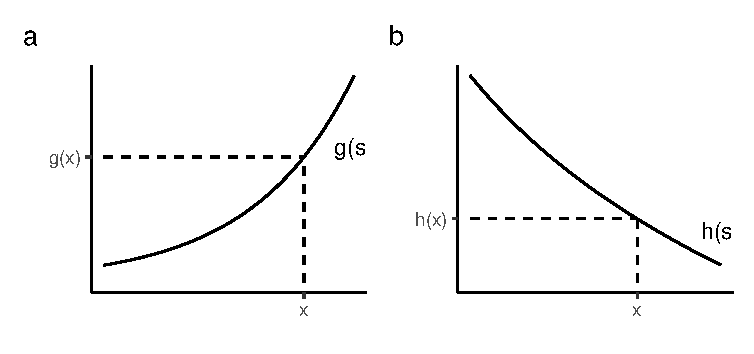
\includegraphics[width=0.95\textwidth]{../graphs/transformation_of_RV}

\caption{Functions of random variables}\label{fig:frv}
\end{figure}



\section{Random vectors}
Given a sample space $\mathcal{C}$. Consider the
two random variables $X_1$ and $X_2$, which assign to each element
$c$ of $\mathcal{C}$ an ordered pair of numbers
$X_1(c)=x_1$, $X_2(c)=x_2$. Then we say that $(X_1,X_2)$ is a
\textbf{random vector}. 

If $(X_1,X_2)$ has density $f_{X_1,X_2}(x_1,x_2)$, the \textbf{marginal density}
of $X_1$ is  $ f_{X_1}(x_1) = \int_{-\infty}^\infty f_{X_1,X_2}(x_1,x_2)\rd x_2$.

If $(X_1,X_2)$ is discrete, then the conditional probability of $X_1$ given $X_2$ is
\[ p_{X_1|X_2}(x_1|x_2) = \frac{p_{X_1,X_2}(x_1,x_2)}{p_{X_2}(x_2)}, \quad \text{where
$p_{X_2}(x_2)>0$}.\] But if $(X_1,X_2)$ is continuous, all point probabilities are
zero, and another way to determine conditional distribution is necessary. It
turns out that if $(X_1,X_2)$ has a density, it is useful to define the
\textbf{conditional density} of $X_1$ given $X_2$ as
\[f_{X_1|X_2}(x_1|x_2)=\frac{f_{X_1,X_2}(x_1,x_2)}{f_{X_2}(x_2)},\quad \text{where $f_{X_2}(x_2)>0$}.\]
With this conditional density, we can define
the \textbf{conditional expectation} is $\E[X_2|X_1=x_1] = \int_{-\infty}^\infty s
f_{X_2|X_1}(s|x_1) \rd s$.

For the completely general case (which we won't be working with), it is useful to first define the \textbf{indicator function}, 
\[ 1_{X\in S} = \begin{cases} 1 & \text{if $X\in S$,} \\ 0 & \text{if $X\notin S$.}\end{cases}\]
and require that for all Borel subsets $S\subset \SR$,
\begin{align*}
  E[P(A|X)\cdot 1_{X\in S}] &= P(A\cap \{X\in S\}),  \\
  E[E[Y|X]\cdot 1_{X\in S}]      &= E[Y\cdot 1_{X\in S}].
\end{align*}
These equations tie down both conditional probability and conditional
expectation.\footnote{With the indicator function, we could have
defined probability as $P(X\in A) = \E[1_{X\in A}]$, this would push the problem
of defining conditional probability into the theory of integration.}




Let $(X_1,X_2)$ have joint d.f. $F(x_1,x_2)$ and let $X_1$ and $X_2$ 
have marginal d.f.s $F_1(x_1)$
  and $F_2(x_2)$. Then $X_1$ and $X_2$ are \textbf{independent} if and only if 
$F(x_1,x_2)= F_1(x_1) F_2(x_2)$. 



Let $(X_1,X_2)$ have joint CDF
  $F(x_1,x_2)$ and let $X_1$ and $X_2$ have marginal CDFs $F_1(x_1)$
  and $F_2(x_2)$. Then $X_1$ and $X_2$ are independent if and only if 
  \[F(x_1,x_2)= F_1(x_1) F_2(x_2),\]
  the joint d.f. being the product of marginal d.f.s. It follows that if the corresponding
  densities exist, $X_1$ and $X_2$ are independent if the joint
  density is the product of marginal densities.

  If $X_1$ and $X_2$ are independent and $\E[u(X_1)]$ and $\E[v(X_2)]$ exist, then
$\E[u(X_1)v(X_2)] = \E[u(X_1)]\cdot \E[v(X_2)]$.



For complete generality, let $Y_1=u_1(X_1,X_2)$ and $Y_2=u_2(X_1,X_2)$ be
one-to-one transformed random variables, and let $w_1$ and $w_2$ be inverses.
Then in general, 
\begin{multline*} \int\!\!\!\int_A f_{X_1,X_2}(x_1,x_2)\rd x_1 \rd x_2 \\
= \int\!\!\!\int_B
f_{X_1,X_2} (w_1(y_1,y_2),w_2(y_1,y_2))| \det(\mathbf{J}(y_1,y_2))| \rd y_1
\rd y_2,\end{multline*} 
where $\mathbf{J}(y_1,y_2)$ is the Jacobian of $\mathbf{w}(\mathbf{y})$ and $B$ is
the image $B=\mathbf{u}(A)$. This is an application of the general formula
for integration with change of variables in calculus.


A vector $\mathbf{X}=(X_1,\dots,X_n)$ where each element is an
\emph{independent} draw from the same distribution as the random variable $X$ is
known as a \textbf{random sample} of size $n$ of the variable $X$.

\section{Estimation}

For estimation, we would like to have some rules to uncover empirical analogs
to theoretically defined parameters. The \textbf{analog principle} is to 
start with a theoretically defined parameter (such as $\mu=\E[X]$) and set its
empirical analog equal to this in the sample. The simple average is is the
empirical analog of an expectation, the sample mean sum square is the empirical
analog of variance and so on. 

For the expectation case, the analog principle is to set $\widehat{\mu} = n^{-1}\sum X_i$,
often written $\overline{X}_n$. For a simple regression model,
\[ Y_i = \alpha + \beta X_i + \varepsilon_i,\] the core assumption is that $\cov[\varepsilon_i,X_i]=0$.
Reformulating, $\cov[Y_i - (\alpha + \beta X_i), X_i]$, or that $\cov[Y_i,X_i] = \beta \var[X_i]$.
The empirical analog of this is that
\[ \widehat{\cov[X_i,Y_i]} = \widehat{\beta} \widehat{\var[X_i]},\]
with the rule that $\widehat{A}$ always mean ``empirical estimate of $A$.'' This equation
is easily solved for $\widehat{\beta} = \widehat{\cov[X_i,Y_i]} / \widehat{\var[X_i]}$. To find
$\widehat{\alpha}$ use the same kind of procedure for the theoretical moment $\E[\varepsilon_i]=0$. This kind
of application of the analog principle is called \textbf{method of moments}. Note
that in this regression case, the assumption $\cov[Y_i - (\alpha + \beta X_i), X_i]$ is equivalent
to the expected first order condition of a least-square minimization.

Often what seems like different approaches end up as equivalent to method of moment estimation.
An example: With \textbf{maximum likelihood}, under some regularity assumptions maximum likelihood 
estimation is equivalent to method of moments with the additional result that the expectation 
of the \textbf{score} (the first order condition of the log likelihood) is zero. But in general,
maximum likelihood is based on maximizing the probability (or density) of the data $L(\mX;\theta)$ 
given the parameters $\widehat{\theta}$. Most of the time, we prefer to maximize the log likelihood,
which for an iid sample is just the sum of individual log likelihoods.

In most of applied economics, we think of the parameters we want to estimate as properties
of some \textbf{data generating process} that potentially can generate infinitely many realizations and
which is inherently stochastic. This tradition goes back to Trygve \citet{Haavelmo1944}.
In survey statistics we instead formulate the problem such that there is a finite population true and
deterministic value, but our estimates are random variables because we only sample a subset of the
full population. Either way, our estimates are random variables, and the study of the stochastic
properties of these random variables is known as \textbf{inference}, which is a crucial input
into hypothesis testing. 

Often we want our estimators to be \textbf{unbiased}, such that
$\E[\widehat{\theta}]=\theta_0$, with $\theta_0$ being the true value. We can
define the \textbf{bias} as $b=\E[\widehat{\theta}] -\theta_0$. Even if
estimators are biased (most non-linear estimators are biased), they can be
\textbf{consistent}. To define consistency we need some asymptotic theory (in
Section~\ref{sec:asymptotics}).

\section{Hypothesis testing}
Assume that we have two alternative ways to think of what might
be true.

The distribution of $X$ is $f(x;\theta)$, with parameter
$\theta\in\Omega$, and our ideas about truth can be described by
regions of $\Omega$:
\[ H_0: \theta\in\omega_0 \quad \text{vs $H_1: \theta\in\omega_1$.}
\]

Our task is, based on a sample from the distribution of $X$, determine
whether to keep on insisting on $H_0$ or reject that in favor of
$H_1$. What we want is often to fix the probability of Type I error
(``significance level'') to $\alpha=0.01,0.05,\dots$, and conditional
on that, minimize probability of type II error. By \textbf{Type I error} we mean that
a null hypothesis is rejected when the null is true; by \textbf{Type II error} we mean
that the null hypothesis is not rejected even though the null is false.

Strictly speaking, we decide on a regions of $(X_1,\dots,X_n)\in C$ in
which to accept or reject $H_0$, but in practice we define
test-statistics $T_n(X_1,\dots,X_n)$ and decide on regions of the test
statistics.
Instead of reporting reject/accept with a given $\alpha$-criterion, papers often report $p$-values (but with
implied fixed $\alpha$). 

\textbf{P-values} are the probability of at least as extreme data given $H_0$,
\[ P( \text{data}| H_0).\]
They do not address the likelihood of $H_0$ being true!
In the classical inference, there are never probabilities attached to hypotheses: Hypotheses are true 
or false, and this is not a sampling issue.
If we want to be Bayesian about hypotheses (have beliefs about them), we need to incorporate the priors: 
\[ P(H_0|\text{data}) = \frac{ P(\text{data}|H_0) P(H_0)}{ P(\text{data}) }. \]
Very little of applied economics is explicitly Bayesian, most is anchored in
\textbf{frequentist inference}. In frequentist philosophy, there is always a
true (but unknown) value of any parameter, and we do not put probabilities on
our beliefs about this parameter. Probabilities are restricted to the
\textbf{sampling distribution} of our estimators \emph{under some null
hypothesis}.

If we assume that $X$ is normally distributed, we could 
test if $E[X] = \mu_0$ using an expression such as
\[
t_n = \frac{\overline{X}_n - \mu_0}{\sigma/\sqrt{n}}.
\]
If we know $\sigma$, then $t_n$ would be normally distributed $N(0,1)$ under $H_0: E[X]=\mu_0$. 
This would be true even in small samples.
We can modify this most simple t-test in various ways.


When we control the type-I error probability to $\alpha$ and the type-II error probability
to $\beta$, we say that we have \textbf{power} $1-\beta$. 
In order to calculate power, it is necessary to be explicit about the alternative hypothesis 
we consider---or calculate for a range of alternative hypotheses. 
Power is the probability of a significant result under the alternative hypothesis, and is a good thing. 
Among people who design experiments, it is customary to aim for power of 80\% or 90\%.

Assume a simple one-sample, one-sided $t$-test against a null-hypothesis of $E[X]=0$. This will
be significant at $\alpha=5\%$ when $t> 1.64$, with probability
\[
P\left( \frac{\overline{X}_n - \mu_0}{\sigma/\sqrt{n}} > 1.64 | E[X]=\mu_1\right) = 
1 - \Phi\left( 1.64 - \frac{\mu_1}{\sigma/\sqrt{n}}\right).
\]
Only the ratio $\mu_1/\sigma$, often known as the \textbf{effect size}  $\delta$, and the sample
size matters.

In Figure~\ref{fig:power} we see the power of a two-sided, two-sample $t$-test
of $\mu=0$ at different alternative hypotheses about the effect size and at
different total sample size. Measuring moderate effect sizes require large sample
sizes to have the power that most consider appropriate (at 0.8 and above). 

\begin{figure}[tb]
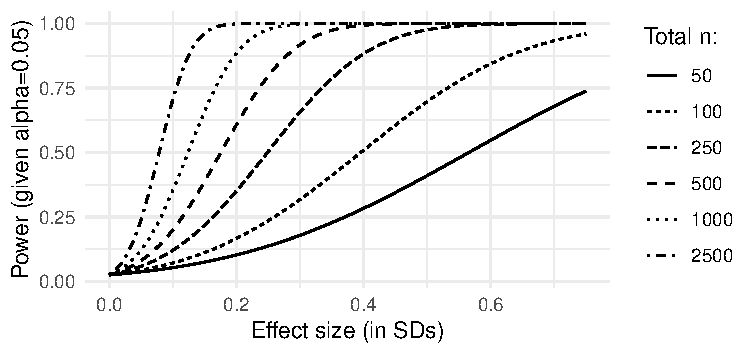
\includegraphics[width=\textwidth]{../graphs/powergraph}

\caption{Power for a two-sided, two-sample $t$-test of $H_0: \mu=0$ as the effect 
size and sample size varies ($\alpha=0.05$)}\label{fig:power}
\end{figure}


If we analyze classical hypothesis testing with Bayesian methods, we can uncover some
unsettling consequences of how low power affects statistical inference. 
Consider Figure~\ref{fig:B}. We encode our prior knowledge as $p$, our belief that
nature made the alternative hypothesis true, while $1-p$ is our belief about
the probability that $H_0$ is true. We cannot observe if we are at the $H_0$ or $H_A$ node,
but if we are at $H_0$ we reject with probability $\alpha$, the level of significance for our
test (a type-I error). If we are at $H_A$, we reject with probability $\gamma$, the power of the
test. Rejecting $H_0$, the Bayesian posterior belief in $H_A$ is
\begin{align*}
   P(H_A|\mathrm{Reject} H_0) & = \frac{P(\mathrm{Reject} H_0|H_A) \cdot P(H_A)}{P(\mathrm{Reject} H_0} \\
   &= \frac{p\gamma}{(1-p)\alpha + p\gamma}.  
\end{align*}

Consider a surprising result ($p=0.1$) in an underpowered study ($\gamma=0.5$), our posterior belief
in $H_A$ should not be very strong: $0.1\cdot 0.5 / (0.9\cdot 0.05 + 0.1\cdot 0.5) = 0.53$.
For this reason there are people who advocate for much stricter $\alpha$: \citet{Benjamin2017} argue
for using $\alpha=0.005$ as a conventional level instead of $0.05$. 

\begin{figure}[tb]
  \begin{center}
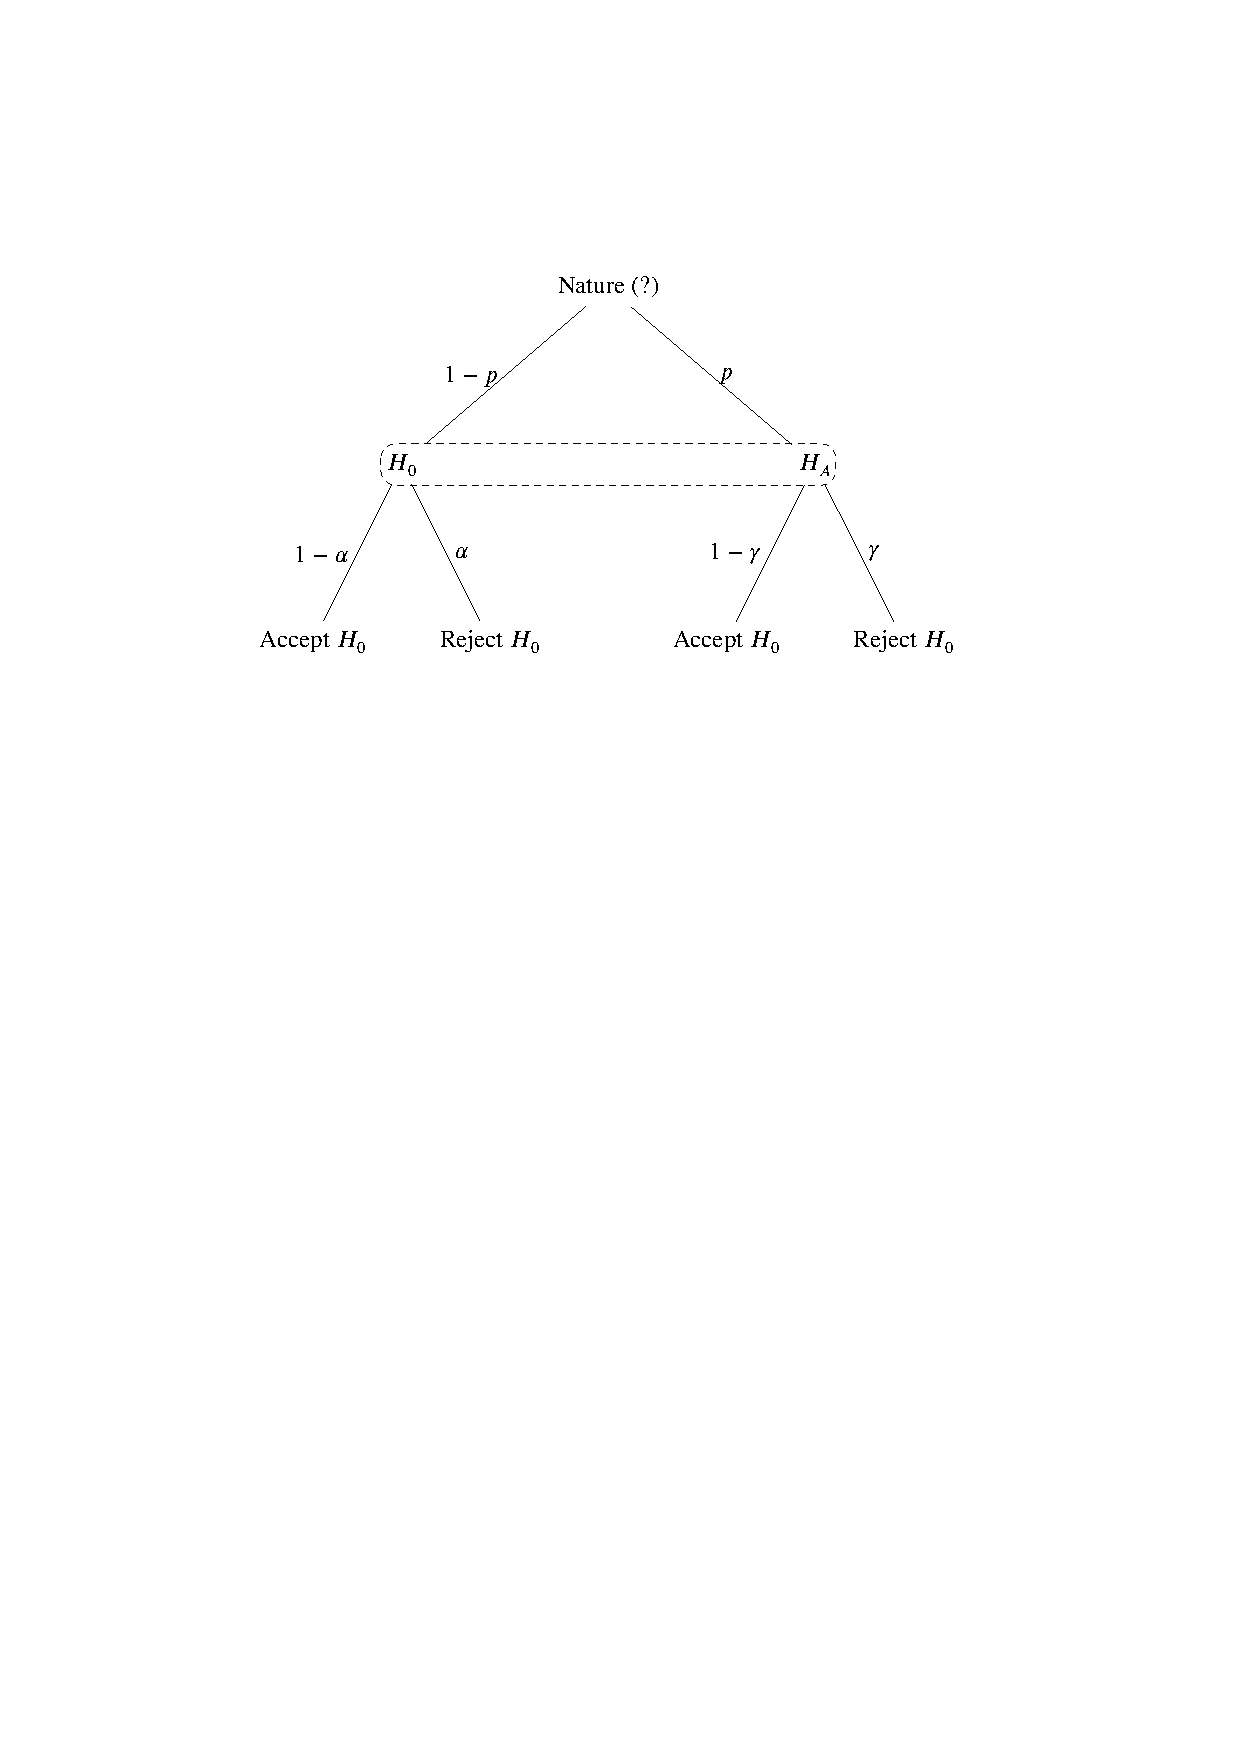
\includegraphics[width=0.8\textwidth]{../graphs/B.pdf}
  \end{center}
\caption{Statistical game tree}\label{fig:B}
\end{figure}


\section{Asymptotic theory}\label{sec:asymptotics}

\subsection{Convergence in probability}

$\{X_n\}$ is a sequence of random variables, and $X$ is a random variable, both
defined on the same sample space. Now $X_n$ \textbf{converges in probability} to $X$
if, for all $\epsilon>0$,
\[\lim_{n\rightarrow\infty} P( |X_n-X|\geq \epsilon) = 0.\] We say that
$\plim X_n = X$, or that $X_n \xrightarrow{P} X$.

\begin{theorem}
Let $\{X_n\}$ be sequence of iid random variables with common mean $\mu$ and
finite variance $\sigma^2$. If $\overline{X}_n = n^{-1}\sum_{i=1}^n X_i$, then
$\plim \overline{X}_n=\mu$. (Weak law of large numbers)
\end{theorem}

There are a number of results about how probability limits work:
\begin{enumerate}
\item Suppose $\plim X_n=X$ and $\plim Y_n=Y$. Then $\plim X_n+Y_n = X+Y$.
\item Suppose $\plim X_n=X$ and $a$ is a constant. Then $\plim a X_n = aX$.
\item Suppose $\plim X_n=a$ and the function $g$ is continuous at $a$. Then $\plim g(X_n)=g(a)$.
\item Suppose $\plim X_n=X$ and $\plim Y_n=Y$, then $\plim X_nY_n=XY$.
\end{enumerate}

The concept of probability limit is closely tied to the statistical concept
of consistency. Let $X$ be a r.v. with d.f. $F(s,\theta)$, for some $\theta\in\Omega$.
Let $X_1,X_2,\dots,X_n$ be a random sample on $X$, and let $T_n$ be a statistic.
$T_n$ is a \textbf{consistent} estimator of $\theta$ if $\plim T_n = \theta$.

\subsection{Convergence in distribution}
$\{X_n\}$ is a sequence of random variables and $X$ is a random variable,
let $F_{X_n}$ and $F_X$ be the respective distribution functions. Let 
$C(F_X)$ be the set of points at which $F_X$ is continuous. Now $X_n$ \textbf{converges in
distribution} to $X$ if $\lim_{n\rightarrow\infty} F_{X_n}(x) = F_X(x)$ for all
$x\in C(F_X)$, and we sometimes write \[X_n \xrightarrow{D} X.\]

Like for convergence in probability, we have some theorems about convergence in distribution:

\begin{enumerate}
\item If $X_n$ converges to $X$ in probability, then $X_n$ converges to $X$ in distribution.
\item If $X_n$ converges to the constant $b$ in distribution, then $X_n$
converges to $b$ in probability.
\item If $X_n$ converges to $X$ in distribution and $Y_n$ converges in probability to $0$,
then $X_n+Y_n$ converges to $X$ in distribution.
\item If $X_n$ converges to $X$ in distribution and $g$ is a continuous function on the support
of $X$, then $g(X_n)$ converges to $g(X)$ in distribution.
\item $X_n$, $X$, $A_n$, and $B_n$ are random variables and $a$ and $b$ are constants. 
If $X_n$ converges to $X$ in distribution, $\plim(A_n)=a$, and $\plim(B_n)=b$, then
\[ A_n + B_n X_n \xrightarrow{D} a + bX.\]
\end{enumerate}


\subsection{The Central Limit Theorem}
There is a whole literature about generalizing central limit theorems. A basic one:

\begin{theorem}
Let $X_1,X_2,\dots,X_n$ denote a random sample from a distribution with mean
$\mu$ and positive variance $\sigma^2$. Then the random variable \[ Y_n =
\left(\sum_{i=1}^n X_i - n\mu \right)/\sqrt{n}\sigma =
\sqrt{n}(\overline{X}_n-\mu)/\sigma\] converges in distribution to a random
variable with a normal distribution $N(0,1)$. 
\end{theorem}

A simple proof can be constructed for the subset of cases where $X$ has a moment generating
function, the trick is to do a second order Taylor-approximation of the moment generating
function of $X-\mu$. 

The $\mathbf{\Delta}$\textbf{-rule} is often useful in conjunction with the CLT.
It says that 

\begin{theorem}
If $\{X_n\}$ is a sequence of random variables such that $\sqrt{n}(\overline{X}_n-\theta)$
converges to $N(0,\sigma^2)$ in distribution, $g$ is a differentiable function at $\theta$,
and $g'(\theta)\neq 0$, then 
\[ \sqrt{n}\left(g(X_n) - g(\theta)\right) \xrightarrow{D} 
N\left(0, \left(g'(\theta)\right)^2\sigma^2\right).\]
\end{theorem}
This can be proven with a Taylor expansion. 

The $\Delta$-rule is the default approach to calculating the distribution of derived
statistics. If we can show that the CLT applies to some moments or parameters,
and we are interested in a function of these moments or parameters, we can use the 
$\Delta$-rule to calculate the distribution of these functions. Statistical packages
will often do this automatically (example: Stata's \texttt{testnl} command).

\section{Selected math facts}
In this section, there are some mathematical facts that turn out to be useful
for probability and statistics but isn't really part of statistics itself.

The \textbf{exponential function}, written $e^s$ or $\exp(s)$ is important. Can be defined by the
series expansion \[ e^x = \sum_{k=0}^\infty \frac{x^k}{k!},\] or
\[ e^x = \lim_{n\rightarrow \infty} \left( 1 + \frac{x}{n} \right)^n. \]
It is also the case that  $\rd e^s / \rd s =e^s$.


If $\psi$ is some function such that $\psi(n) \rightarrow 0$ as $n\rightarrow\infty$,
then \[ \lim_{n\rightarrow\infty} \left(1 + \frac{x}{n} + \frac{\psi(n)}{n}  \right)^n = e^x,\]
since the $\psi(n)/n$ term vanishes faster than $x/n$.

A useful formulation of \textbf{Taylor's formula} is that for continuous and at
least twice differentiable functions functions $m\!\!\!:\!\!\SR \rightarrow \SR$, there
exists a number $\xi$ between $0$ and $t$ such that \[ m(t) = m(0) + m'(0) t +
\frac{1}{2} m''(\xi) t^2.\]


\section{Some calculating rules for $P$, $\E$, $\var$ and $\cov$}
Let $A$ and $B$ be some events; $X$, $Y$, and $Z$ are random variables.
\begin{enumerate}
\item $P(A) = 1 - P(A^c)$.
\item $P(A) = P(A\cap B) + P(A\cap B^c)$.
\item $P(A\cup B) = P(A) + P(B) - P(A\cap B)$.
\item $P(A\cap B) \leq \min\{P(A), P(B)\}$.
\item $P(A \cap B) = P(A)P(B|A)$.
\item $\E\left[\E[Y|X]\right] = \E[Y]$.
\item $\E[a + bX ] = a + b\E[X]$.
\item $\E[a X + b Y] = a\E[X] + b\E[Y]$.
\item $\E[g(X)] = \int g(x) f_X(x) \rd x$.
\item $\E[XY] = \E[X]\E[Y]$ but only when $X$ and $Y$ are \emph{independent}!
\item $\E[|X+Y|] \leq \E[|X|] + E[|Y|]$.
\item $\var[X] = \E[X^2] - \left(E[X]\right)^2$.
\item $\var[\overline{X}_n] = \sigma^2 / n$.
\item $\cov[X,Y] = \E[XY] - \E[X]\E[Y]$.
\item $\cov[X,X] = \var[X]$.
\item $\var[a + bX] = b^2 \var[X]$.
\item $\var[a X + b Y] = a^2 \var[X] + b^2 \var[Y] + 2 a b \cov[X,Y]$, note the consequence when $b$ is negative.
\item $\cov[X+Y,Z] =  \cov[X,Z] + \cov[Y,Z]$.
\item $\cov[g(X),X] = \E[g(X)X]  - \E[g(X)]\E[X]$.
\end{enumerate}

\newpage
\addcontentsline{toc}{section}{References}
\bibliographystyle{standard3}
\bibliography{mmref}

\clearpage

\begin{table}
  \caption{Standard normal distribution table}\label{tab:z}

  \medskip
\begin{footnotesize}
  \begin{tabular}{rrrrrrrrrrr} 
    \toprule
      & \multicolumn{10}{c}{Add to $z$ to find $\Phi(z)$} \\
       \cmidrule(lr){2-11}
    $z$ & 0.00 & 0.01 & 0.02 & 0.03 & 0.04 & 0.05 & 0.06 & 0.07 & 0.08 & 0.09 \\ 
    \midrule
    0.0 & $0.500$ & $0.504$ & $0.508$ & $0.512$ & $0.516$ & $0.520$ & $0.524$ & $0.528$ & $0.532$ & $0.536$ \\ 
    0.1 & $0.540$ & $0.544$ & $0.548$ & $0.552$ & $0.556$ & $0.560$ & $0.564$ & $0.567$ & $0.571$ & $0.575$ \\ 
    0.2 & $0.579$ & $0.583$ & $0.587$ & $0.591$ & $0.595$ & $0.599$ & $0.603$ & $0.606$ & $0.610$ & $0.614$ \\ 
    0.3 & $0.618$ & $0.622$ & $0.626$ & $0.629$ & $0.633$ & $0.637$ & $0.641$ & $0.644$ & $0.648$ & $0.652$ \\ 
    0.4 & $0.655$ & $0.659$ & $0.663$ & $0.666$ & $0.670$ & $0.674$ & $0.677$ & $0.681$ & $0.684$ & $0.688$ \\ 
    \addlinespace[2pt]
    0.5 & $0.691$ & $0.695$ & $0.698$ & $0.702$ & $0.705$ & $0.709$ & $0.712$ & $0.716$ & $0.719$ & $0.722$ \\ 
    0.6 & $0.726$ & $0.729$ & $0.732$ & $0.736$ & $0.739$ & $0.742$ & $0.745$ & $0.749$ & $0.752$ & $0.755$ \\ 
    0.7 & $0.758$ & $0.761$ & $0.764$ & $0.767$ & $0.770$ & $0.773$ & $0.776$ & $0.779$ & $0.782$ & $0.785$ \\ 
    0.8 & $0.788$ & $0.791$ & $0.794$ & $0.797$ & $0.800$ & $0.802$ & $0.805$ & $0.808$ & $0.811$ & $0.813$ \\ 
    0.9 & $0.816$ & $0.819$ & $0.821$ & $0.824$ & $0.826$ & $0.829$ & $0.831$ & $0.834$ & $0.836$ & $0.839$ \\ 
    \addlinespace[2pt]
    1.0 & $0.841$ & $0.844$ & $0.846$ & $0.848$ & $0.851$ & $0.853$ & $0.855$ & $0.858$ & $0.860$ & $0.862$ \\ 
    1.1 & $0.864$ & $0.867$ & $0.869$ & $0.871$ & $0.873$ & $0.875$ & $0.877$ & $0.879$ & $0.881$ & $0.883$ \\ 
    1.2 & $0.885$ & $0.887$ & $0.889$ & $0.891$ & $0.893$ & $0.894$ & $0.896$ & $0.898$ & $0.900$ & $0.901$ \\ 
    1.3 & $0.903$ & $0.905$ & $0.907$ & $0.908$ & $0.910$ & $0.911$ & $0.913$ & $0.915$ & $0.916$ & $0.918$ \\ 
    1.4 & $0.919$ & $0.921$ & $0.922$ & $0.924$ & $0.925$ & $0.926$ & $0.928$ & $0.929$ & $0.931$ & $0.932$ \\ 
    \addlinespace[2pt]
    1.5 & $0.933$ & $0.934$ & $0.936$ & $0.937$ & $0.938$ & $0.939$ & $0.941$ & $0.942$ & $0.943$ & $0.944$ \\ 
    1.6 & $0.945$ & $0.946$ & $0.947$ & $0.948$ & $0.949$ & $0.951$ & $0.952$ & $0.953$ & $0.954$ & $0.954$ \\ 
    1.7 & $0.955$ & $0.956$ & $0.957$ & $0.958$ & $0.959$ & $0.960$ & $0.961$ & $0.962$ & $0.962$ & $0.963$ \\ 
    1.8 & $0.964$ & $0.965$ & $0.966$ & $0.966$ & $0.967$ & $0.968$ & $0.969$ & $0.969$ & $0.970$ & $0.971$ \\ 
    1.9 & $0.971$ & $0.972$ & $0.973$ & $0.973$ & $0.974$ & $0.974$ & $0.975$ & $0.976$ & $0.976$ & $0.977$ \\ 
    \addlinespace[2pt]
    2.0 & $0.977$ & $0.978$ & $0.978$ & $0.979$ & $0.979$ & $0.980$ & $0.980$ & $0.981$ & $0.981$ & $0.982$ \\ 
    2.1 & $0.982$ & $0.983$ & $0.983$ & $0.983$ & $0.984$ & $0.984$ & $0.985$ & $0.985$ & $0.985$ & $0.986$ \\ 
    2.2 & $0.986$ & $0.986$ & $0.987$ & $0.987$ & $0.987$ & $0.988$ & $0.988$ & $0.988$ & $0.989$ & $0.989$ \\ 
    2.3 & $0.989$ & $0.990$ & $0.990$ & $0.990$ & $0.990$ & $0.991$ & $0.991$ & $0.991$ & $0.991$ & $0.992$ \\ 
    2.4 & $0.992$ & $0.992$ & $0.992$ & $0.992$ & $0.993$ & $0.993$ & $0.993$ & $0.993$ & $0.993$ & $0.994$ \\ 
    \addlinespace[2pt]
    2.5 & $0.994$ & $0.994$ & $0.994$ & $0.994$ & $0.994$ & $0.995$ & $0.995$ & $0.995$ & $0.995$ & $0.995$ \\ 
    2.6 & $0.995$ & $0.995$ & $0.996$ & $0.996$ & $0.996$ & $0.996$ & $0.996$ & $0.996$ & $0.996$ & $0.996$ \\ 
    2.7 & $0.997$ & $0.997$ & $0.997$ & $0.997$ & $0.997$ & $0.997$ & $0.997$ & $0.997$ & $0.997$ & $0.997$ \\ 
    2.8 & $0.997$ & $0.998$ & $0.998$ & $0.998$ & $0.998$ & $0.998$ & $0.998$ & $0.998$ & $0.998$ & $0.998$ \\ 
    2.9 & $0.998$ & $0.998$ & $0.998$ & $0.998$ & $0.998$ & $0.998$ & $0.998$ & $0.999$ & $0.999$ & $0.999$ \\ 
    \bottomrule
    \end{tabular}
  \end{footnotesize}

    \medskip
    \emph{Note:} To calculate $\Phi(z)$ for $z\geq0$, find the row using the
    first decimal in $z$, and find the second decimal to find the correct
    column. For $z<0$, use the symmetry of the distribution to find  $\Phi(z) =
    1-\Phi(-z)$. The table is calculated with the R-function \texttt{pnorm} \citep{R2023}.
\end{table}



\end{document}